\documentclass[12 pt]{beamer}
\usetheme[
  bullet=circle,		% Other option: square
  bigpagenumber,		% circled page number on lower right
  topline=true,			% colored bar at the top of the frame 
  shadow=false,			% Shading for beamer blocks
  watermark=BG_lower,	% png file for the watermark
]{Flip}


\newcommand{\titleimage}{title}			% Custom title 
\newcommand{\tanedo}{tanedolight}		% Custom author name
\newcommand{\CMSSMDM}{CMSSMDMlight.png}	% light background plot


%%%%%%%%%%
% FONTS %
%%%%%%%%%%

\usepackage[T1]{fontenc}
%\usepackage{lmodern}		
%\usepackage{sfmath}		% Sans Serif Math, off by default

%% Protects fonts from Beamer screwing with them
%% http://tex.stackexchange.com/questions/10488/force-computer-modern-in-math-mode
\usefonttheme{professionalfonts}


\usepackage[no-math]{fontspec}		

%\defaultfontfeatures{Mapping=tex-text}	% This seems to be important for mapping glyphs properly

\usepackage{amsmath}
%\usepackage{amsfonts}
%\usepackage{amssymb}
\usepackage{mathspec}
\usepackage{graphicx}
%\usepackage{mathrsfs} 			% For Weinberg-esque letters
\usepackage{cancel}				% For "SUSY-breaking" symbol
\usepackage{slashed}            % for slashed characters in math mode
%\usepackage{bbm}                % for \mathbbm{1} (unit matrix)
\usepackage{amsthm}				% For theorem environment
\usepackage{multirow}			% For multi row cells in table
\usepackage{arydshln} 			% For dashed lines in arrays and tables
\usepackage{tikzfeynman}		% For Feynman diagrams
% \usepackage{subfig}           % for sub figures
% \usepackage{young}			% For Young Tableaux
% \usepackage{xspace}			% For spacing after commands
% \usepackage{wrapfig}			% for Text wrap around figures
% \usepackage{framed}

\usepackage{setspace}

\setsansfont{calibri}[ 
Extension = .ttf,
UprightFont = *,
BoldFont = *b,
ItalicFont = *i,
Scale = 1
]

\setmathfont(Digits,Latin,Greek){SitkaI.ttc}

\graphicspath{{images/}}	% Put all images in this directory. Avoids clutter.


\usetikzlibrary{backgrounds}
\usetikzlibrary{mindmap,trees}	% For mind map
\usetikzlibrary{arrows,positioning,calc}
\usetikzlibrary{shapes}
% http://www.texample.net/tikz/examples/computer-science-mindmap/


% SOME COMMANDS THAT I FIND HANDY
% \renewcommand{\tilde}{\widetilde} % dinky tildes look silly, dosn't work with fontspec
\newcommand{\comment}[1]{\textcolor{comment}{\footnotesize{#1}\normalsize}} % comment mild
\newcommand{\Comment}[1]{\textcolor{Comment}{\footnotesize{#1}\normalsize}} % comment bold
\newcommand{\COMMENT}[1]{\textcolor{COMMENT}{\footnotesize{#1}\normalsize}} % comment crazy bold
\newcommand{\Alert}[1]{\textcolor{Alert}{#1}} % louder alert
\newcommand{\ALERT}[1]{\textcolor{ALERT}{#1}} % loudest alert
%% "\alert" is already a beamer pre-defined



\author{}
\title{Informatikai Rendszerek Biztonságtechnikája}
\institute{}
\date{}



\begin{document}

%% To use external nodes; http://www.texample.net/tikz/examples/beamer-arrows/
\tikzstyle{every picture}+=[remember picture]

{
  \setbeamertemplate{sidebar right}{\llap{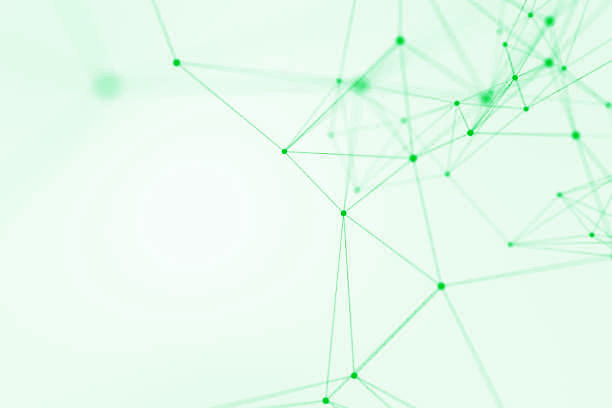
\includegraphics[width=\paperwidth,height=\paperheight]{backgnd}}}

  \begin{frame}[c]
    \begin{center}
      % \includegraphics[width=7cm]{WarpedPenguinsReturn}

      \Large
      \textbf{Információs rendszerek}

      \textbf{biztonságtechnikája}

      \qquad

      Kriptográfia

      Nyilvános kulcsú algoritmusok

      \qquad

      \textit{Vakulya Gergely}

    \end{center}
  \end{frame}
}

  %------------------------------------------------

\begin{frame}{A nyilvános kulcsú titkosítás elve}
    \begin{itemize}
      \item{A szimmetrikus kulcsú titkosítással szemben külön titkosító és kititkosító kulcs.}
      \item{A két kulcs együtt kerül létrehozásra.}
      \item{A két kulcs közül az egyiket nyilvánosságra hozom (nyilvános kulcs, public key).}
      \item{A másikat titkosan kezelem (titkos kulcs, private key).}
      \item{Ha valaki nekem szeretne üzenetet küldeni, az üzenetet az \textbf{én nyilvános kulcsommal titkosítja}.}
      \item{Ezt az üzenetet \textbf{csak én tudom megfejteni} az én \textbf{titkos kulcsommal}.}
      \item{A gyors működés jellemzően nem elsődleges követelmény.}
    \end{itemize}
\end{frame}

\begin{frame}{Az RSA titkosítás}
  \begin{itemize}
    \item{Ron Rivest, Adi Shamir és Len Adleman, 1976}
    \item{Az algoritmus arra épül, hogy a prímszámok szorzatára való felbontásra (faktorizációra) nem ismert gyors algoritmus.}
    \item{Az algoritmus vázlata:}
      \begin{itemize}
        \item{Választunk két különböző, nagy (többszáz jegyű), \textbf{véletlenszerű} prímszámot ($p, q$).}
        \item{Kiszámítjuk a prímek szorzatát ($N = p \cdot q$). Fontos: $N$-ből $p$-t és $q$-t nagyon nehéz megkapni.}
        \item{Kiszámítjuk az $N$ Euler-függvényét: $\varphi(N) = (p-1) \cdot (q-1)$.}
        \item{Választunk egy $\varphi(N)$-hez relatív prím $e$ számot. (Például egy prímszám megfelel, szokásos értékek: 3, 65537.)}
        \item{Kiszámítjuk $d$-t, $e$ modulo $\varphi(N)$ inverzét, tehát egy olyan számot, amire: $e \cdot d \equiv 1 \mod \varphi(N)$.}
        \item{Nyilvános kulcs: $(N, e)$, titkos kulcs: $d$}
        \item{Kódolás: $c = p^e \mod N$}
        \item{Dekódolás: $p = c^d \mod N$}
      \end{itemize}
  \end{itemize}
\end{frame}

\begin{frame}{A prímszámok előállítása}
  \begin{itemize}
    \item{Az RSA algoritmus alapja a nagy méretű, véletlenszerű prímszámok előállítása.}
    \item{A kiindulási alap: véletlenszámok előállítása. Kiválasztás: Prímtesztek.}
    \item{A legtöbb prímteszt nem garantál prímszámokat, de ennek valószínűsége tetszőlegesen nagy lehet.}
    \item{Fontos, hogy a prímszámokat ne használjuk fel újra.}
    \item{Fontos a véletlenszámok minősége.}
    \item{\href{https://www.cve.org/CVERecord?id=CVE-2008-0166}{CVE-2008-0166}}
    \item{\href{https://github.com/g0tmi1k/debian-ssh}{CVE-2008-0166 összefoglaló}}
  \end{itemize}
\end{frame}

\begin{frame}{Két matematikai kérdés az RSA-val kapcsolatban}
  \begin{block}{Prímfaktorizáció}
    \begin{itemize}
      \item{Az RSA biztonsága a prímfaktorizációban rejlik. Ha a kulcsgeneráláskor kapott szorzatot faktorizálni tudjuk,
        kiszámíthatjuk a titkos kulcsot.}
      \item{Ez a faktorizáció általános esetben NP nehézségű, de valószínűleg nem NP-teljes.}
      \item{NP = Non-Polinomial? Nem!}
      \item{NP = Nondeterministic Polinomial? Igen!}
      \item{A kvantumszámítógépek komoly fejtörést okozhatnak.}
    \end{itemize}
  \end{block}

  \begin{block}{Modulo-$n$ hatványozás}
    \begin{itemize}
      \item{A kódolás és dekódolás (modulo $n$) hatványozást használ.}
      \item{Ez ismételt szorzással valósítható meg.}
      \item{A végrehajtási időkből következtetni lehet a kulcsra.}
    \end{itemize}
  \end{block}
\end{frame}

\begin{frame}{Nyilvános kulcsok továbbítása}
  \begin{itemize}
    \item{Az RSA nagy bizonságot garantál.}
    \item{Viszont számításigényes.}
    \item{A blokk kódolók bitekkel dolgoznak, rajtuk logikai műveleteket hajtanak végre.}
    \item{Az RSA számokon hajt végre matematikai műveleteket (modulo $n$ hatványozást).}
    \item{Minden üzenetet egyetlen számmá kell transzformálni az RSA-val való titkosításhoz.}
    \item{Így az RSA célszerűtlen hosszabb üzenetek továbbítására.}
    \item{Megoldás: RSA-val csak egy blokk kódolóhoz használatos kulcsot küldjük át, maga a kommunikáció
      már a (sokkal gyorsabb) blokk kódolóval történik.}
  \end{itemize}
\end{frame}

\begin{frame}{A Diffie-Hellman kulcscsere}
  \begin{itemize}
    \item{Szimmetrikus kulcsú titkosító algoritmus kulcsai más módszerrel is megoszthatóak a partnerek között.}
    \item{A Diffie-Hellman kulcscsere lényege, hogy nem egy, az egyik partnernek már birtokában levő kulcsot küld el a másik partnernek}
    \item{Ehelyett \textbf{közösen hoznak létre} egy \textbf{megosztott titkot} (shared secret).}
    \item{Harmadik fél az összes üzenet lehallgatásával sem tudja a megosztott titkot létrehozni.}
    \item{A konkrét megvalósításokban nem maga a megosztott titok a kulcs, hanem abból valamilyen hash algoritmussal van származtatva.}
  \end{itemize}
\end{frame}
\begin{frame}{D-H alalógia}
  \begin{itemize}
    \item{Analógia:}
      \begin{itemize}
        \item{Alice elküld egy aktatáskát Bobnak, amit egy lakattal zár le. Ehhez a lakathoz csak Alice-nak van kulcsa.}
        \item{Bob nem tudja kinyitni a táskát, mert azon lakat van, viszont ő is le tudja zárni. Bob tehát szintén tesz a táskára egy lakatot, amihez csak neki van kulcsa, majd visszaküldi Alice-nak a duplán lelakatolt táskát.}
        \item{Alice kinyitja és leveszi a saját lakatját, majd visszaküldi a táskát Bobnak.}
        \item{Bob kinyitja és leveszi a lakatot, így ki tudja nyitni a táskát.}
      \end{itemize}
    \item{A Diffie-Helmann kucscsere alapja az RSA-hoz hasonlóan egy olyan kát olyan művelet, amik kioltják egymást.}
  \end{itemize}
\end{frame}

\begin{frame}{A digitális aláírás}
  \begin{itemize}
    \item{Az RSA titkosításnál a kódolás és a dekódolás művelete gyakorlatilag azonos, csak a kulcs más.}
    \item{A titkos kulccsal is lehet kódolni és a nyilvános kulccsal is lehet dekódolni.}
    \item{Mi értelme úgy kódolni valamit, hogy bárki visszafejtheti? Ezzel tudja bizonyítani valaki, hogy ő küldte az üzenetet.}
    \item{A digitális aláírás lényege:}
      \begin{itemize}
        \item{Generálunk egy kulcspárt. A publikus kulcsot mindenki rendelkezésére bocsájtjuk.}
        \item{Az aláírandó üzenetből hash-t képezünk.}
        \item{A hash-t a \textbf{titkos} kulcsunkkal titkosítjuk. Ennek eredménye lesz a digitális aláírás.}
        \item{A címzett a hash-t kititkosítja a mi \textbf{nyilvános} kulcsunkkal, majd összeveti a vett üzenet hash-ével.}
      \end{itemize}
  \end{itemize}
\end{frame}

\begin{frame}{Digitális tanúsítványok}
  \begin{itemize}
    \item{Az üzeneteket digitális aláírással láthatjuk el. De mi van, ha valaki más is készít egy kulcspárt a mi nevünkben és ezt aláírásra használja?}
    \item{Erre jelent megoldást a digitális tanúsítvány (certificate).}
    \item{A tanúsítványt a tanúsító hatóság (certificate authority, CA) állítja ki.}
    \item{A tanúsítvány részei:}
      \begin{itemize}
        \item{A tanúsítvány tulajdonosának adatai}
        \item{A tulajdonos publikus kulcsa}
        \item{Érvényességi idő}
        \item{A tanúsítvány kiállítója}
        \item{A kiállító digitális aláírása}
      \end{itemize}
    \item{A CA-ban mindkét résztvevő megbízik.}
    \item{A tanúsítvány (ami a nyilvános kulcs hitelességét bizonyítja) a CA nyilvános kulcsával ellenőrizhető.}
  \end{itemize}
\end{frame}

\begin{frame}{A bizalmi lánc (chain of trust)}
  \begin{itemize}
    \item{Egyetlen CA csak korlátozott számú tanúsítványt képes kiadni.}
    \item{Megoldás: Bizalmi hierarchia (fa struktúrával).}
    \item{Az egyes CA-k saját tanúsítványai a felettük levő szinten levő CA-ra hivatkozhatnak.}
    \item{A hierarchia tetején a root CA áll. Root CA-ből több is van, többféle bizalmi lánc is létezhet párhuzamosan.}
    \item{A nyilvános kulcsú tanúsítványokat az X.509 szabvány definiálja.}
  \end{itemize}
\end{frame}

\begin{frame}{Nyílt kulcsú titkosítási szabványok (Public-Key Cryptography Standards, PKCS)}
  Bizonyos célra ajánlott titkosítási szabványok gyűjteménye
    \begin{itemize}
      \item{PKCS \#1: RSA}
      \item{PKCS \#3: Diffie-Helman kulcscsere}
      \item{PKCS \#5: Jelszó alapú titkosítás (PBKDF2)}
      \item{PKCS \#7: Digitális aláírások és tanúsítványok}
      \item{PKCS \#8: Titkos kulcsok tárolása}
      \item{PKCS \#10: Tanúsítványkérelmek}
      \item{PKCS \#12: Kriptográfiai fájlok tárolása}
    \end{itemize}
\end{frame}

\end{document}
